\documentclass{article}

\usepackage{ctex}

\usepackage{enumerate}
\usepackage{amsthm}
\usepackage{amssymb}
\usepackage{bm}
\usepackage{geometry}
\usepackage{amsmath}
\usepackage{mathrsfs}
\geometry{
    a4paper,
    left=20mm,
    right=20mm,
    top=20mm,
    }
\usepackage{mathtools}
\mathtoolsset{showonlyrefs=true}
\newtheorem{thm}{Theorem}[subsection]

\newtheorem{Prob}{Theorem}[section]
\newtheorem{Lem}{Lemma}[section]

\usepackage{xcolor}
\usepackage{graphicx}
\usepackage{hyperref}
\hypersetup{
    colorlinks=true,
    linkcolor=blue,
    filecolor=magenta,
    urlcolor=red,
}
\urlstyle{same}

%%% Declare %%%
\newcommand{\md}{\mathrm{d}}
\newcommand{\mR}{\mathbb{R}}
\newcommand{\trans}{\mathsf{T}}
\newcommand{\me}{\mathrm{e}}
\newcommand{\mi}{\mathrm{i}}
%%% Declare %%%

%%% custom %%%
\newcommand{\mM}{\mathcal{M}}
\newcommand{\mH}{\mathcal{H}}
\newcommand{\mA}{\mathcal{A}}
\newcommand{\mF}{\mathcal{F}}
\newcommand{\mX}{\mathcal{X}}
\newcommand{\mY}{\mathcal{Y}}
\newcommand{\mZ}{\mathcal{Z}}
\newcommand{\mO}{\mathcal{O}}
\newcommand{\mE}{\mathcal{E}}
\newcommand{\mbE}{\mathbb{E}}
\newcommand{\mD}{\mathcal{D}}
\newcommand{\mS}{\mathcal{S}}

\DeclareMathOperator*{\argmin}{argmin}

%%$ custom %%%
\usepackage[all]{xy}

%%% document info %%%
\title{Latent Assimilation with Implicit Neural Representations (LAINR)}
\author{李卓远\hspace*{5ex}数学科学学院}
\date{\href{mailto:zy.li@stu.pku.edu.cn}{zy.li@stu.pku.edu.cn}}
%%%


\begin{document}
\maketitle
\section{Motivation for Latent Assimilation}
\subsection{Data Assimilation}
资料同化(data assimilation)广泛存在于气象学、海洋学、地球物理学等领域,其目的是通过观测数据来修正模型的状态,从而提高模型的预测能力.
\begin{figure}\label{fig:da-pipeline}
	\centering
	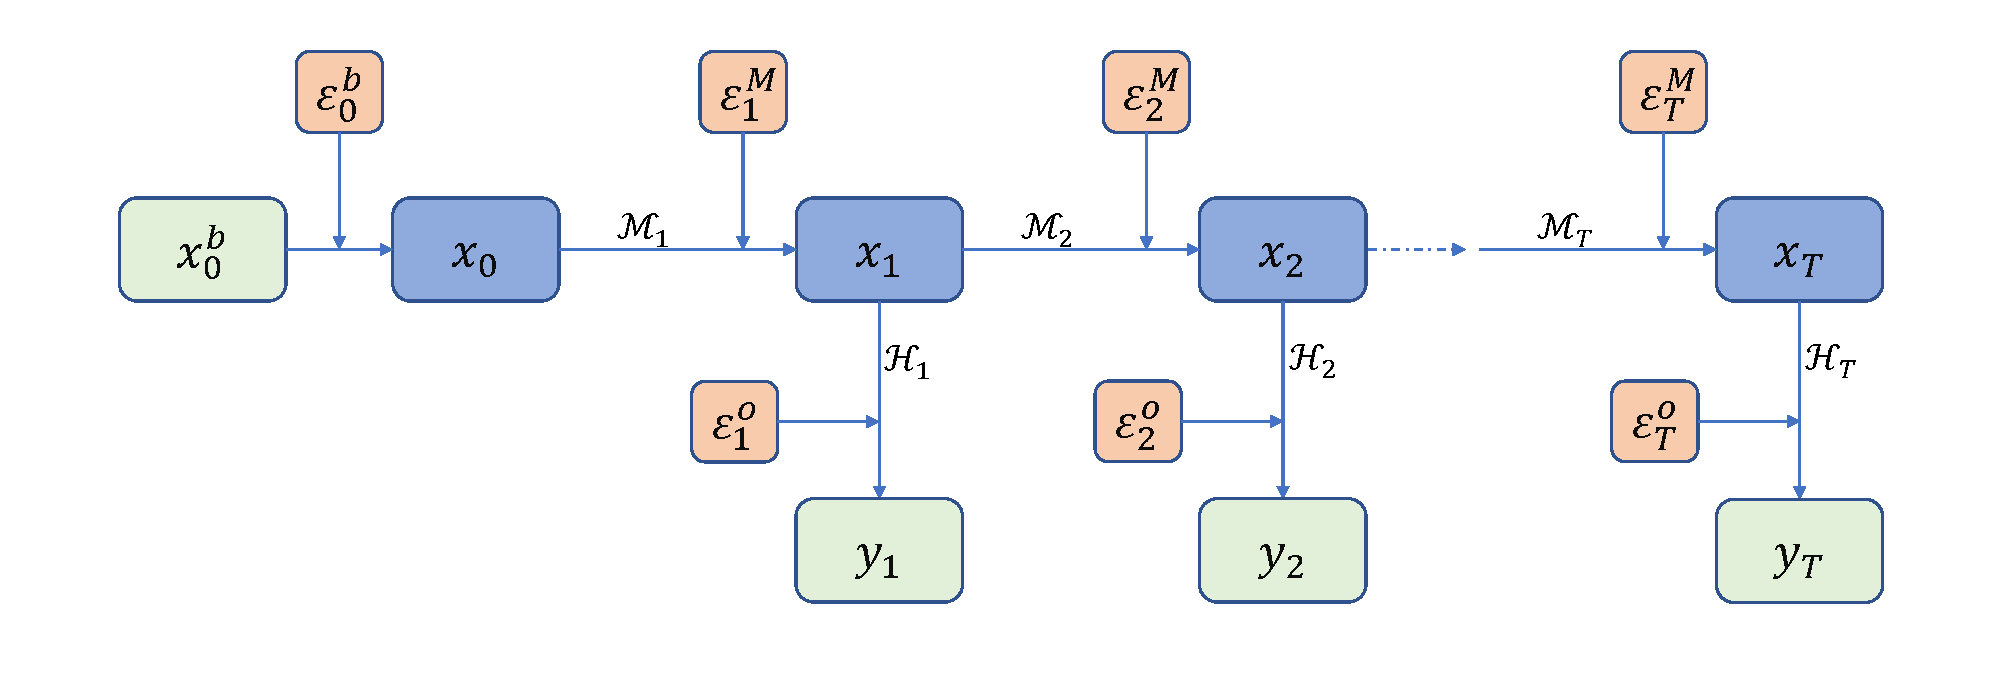
\includegraphics[width=.8\textwidth]{figs/4d-var-pipeline.pdf}
	\caption{DA pipeline}
\end{figure}
如图 \ref{fig:da-pipeline} 所示,其中$x_{0\sim T}$表示模型状态(model states),例如整个大气系统在每个格点处的状态之集,其演化过程用$\mM$表示. 而$y_{1\sim T}$指代每个时刻对当前系统的一个观测,例如在实际应用中可以是气象卫星和气象站等实际观测数据.除此之外, $x_0^b$是我们对于初始场$x_0$的某个估计.由于实际建模和观测总会包含难以消除的误差,在资料同化计算中还需考虑这些误差带来的影响.为叙述方便,以下记$\mX$和$\mY$分别为模型状态空间和观测空间.
\subsection{Reduce-order Model and Latent Assimilation}
在传统的资料同化方法中,模型的状态空间往往非常庞大($\dim\mX\sim\mO(10^7)$),模型状态$x_{0\sim T}$通常表现为一个相当高维的向量,因此设计相关算法往往受限于模型状态空间的维数.为了解决这个问题,一个基本的假设是虽然模型状态所在的空间维数很高,但受限于物理定律,其实际取值往往落在一个低维子流形上$\mX'\subseteq\mX$,其中$\dim\mX'\ll\dim\mX$.因此我们考虑利用降阶模型(reduce-order models)和压缩的方式将$\mX'$与一个低维隐空间(latent space) $\mZ$建立一个一一对应的关系.将已有成熟的DA算法平行地迁移到latent space进行相关操作.在本文中我们称latent space上的assimilation为latent assimilation.
\[
	\xymatrix{
		\mX\ar[r]^{\mM}\ar[d]_{\mH}&\mX\ar[d]^{\mH}\\
		\mY&\mY
	}
	\Rightarrow
	\xymatrix{
		\mZ\ar[r]^{g}\ar[d]^{\mD}&\mZ\ar[d]^{\mD}\\
		\mX\ar[u]^{\mE}\ar[r]^{\mM}\ar[d]_{\mH}&\mX\ar[u]^{\mE}\ar[d]^{\mH}\\
		\mY&\mY
	}
\]
事实上传统方法也试图使用PCA等确定性方法对模型状态进行降维,但这类方法往往会丢失模型状态自身的物理信息,隐空间的动力学演化过程往往只能通过粗糙的线性回归进行处理,同时对于小尺度的特征也难以重建.因此我们考虑利用神经网络对模型状态进行降维,提高压缩精度的同时还能学到较为精确的隐空间上的物理规律.
\section{Latent Assimilation with Encoder-Decoder}
\subsection{description}
在2021年, Peyron等人\cite{Peyron2021LAwithAE}提出使用类似Encoder-Decoder的结构将模型投射到隐空间中,其选取的实验模型是Lorenz-96.首先固定一个非线性映射$\mR^{40}\to\mR^{400}$,将原本40维的Lorenz-96模拟数据转变为$\mR^{400}$中.然后基于这些存在于400维空间中的数据进行同化.核心思想概括如下:
\begin{itemize}
	\item 构造多层全连接神经网络$\mE_\theta:\mR^{400}\to\mR^{40}$和$\mD_\theta:\mR^{40}\to\mR^{400}$使得$\mD_\theta\circ\mE_\theta$在$\mX'$上为恒等映射.
	\item 在隐空间$\mR^{40}$中建立一个RNN模型$g_\phi$,具体构架借鉴了ReZero\cite{bachlechner2021rezero}的思想,训练网络参数使其满足$\mM=\mD_\theta\circ g_\phi\circ\mE_\theta$.
	\item 网络结构如图 \ref{fig:Peyron2021-structure} 所示,使用的训练损失函数为
	      \[L=\mbE_{x_{0\sim s}}\sum_{k=1}^s\|\mD_\theta\circ\mE_\theta(x_k)-x_k\|^2+\lambda\|\mD_\theta\circ g_\phi^k\circ\mE_\theta(x_0)-x_k\|^2,\]
	      其中超参数$s=2$, $\lambda=5.0$.
	\item 最后在隐空间上使用ETKF-Q算法(实为IEnKS-Q\cite{Fillion2020IEnKS}的一个特例)得到相应的结果.
\end{itemize}
\begin{figure}\label{fig:Peyron2021-structure}
	\centering
	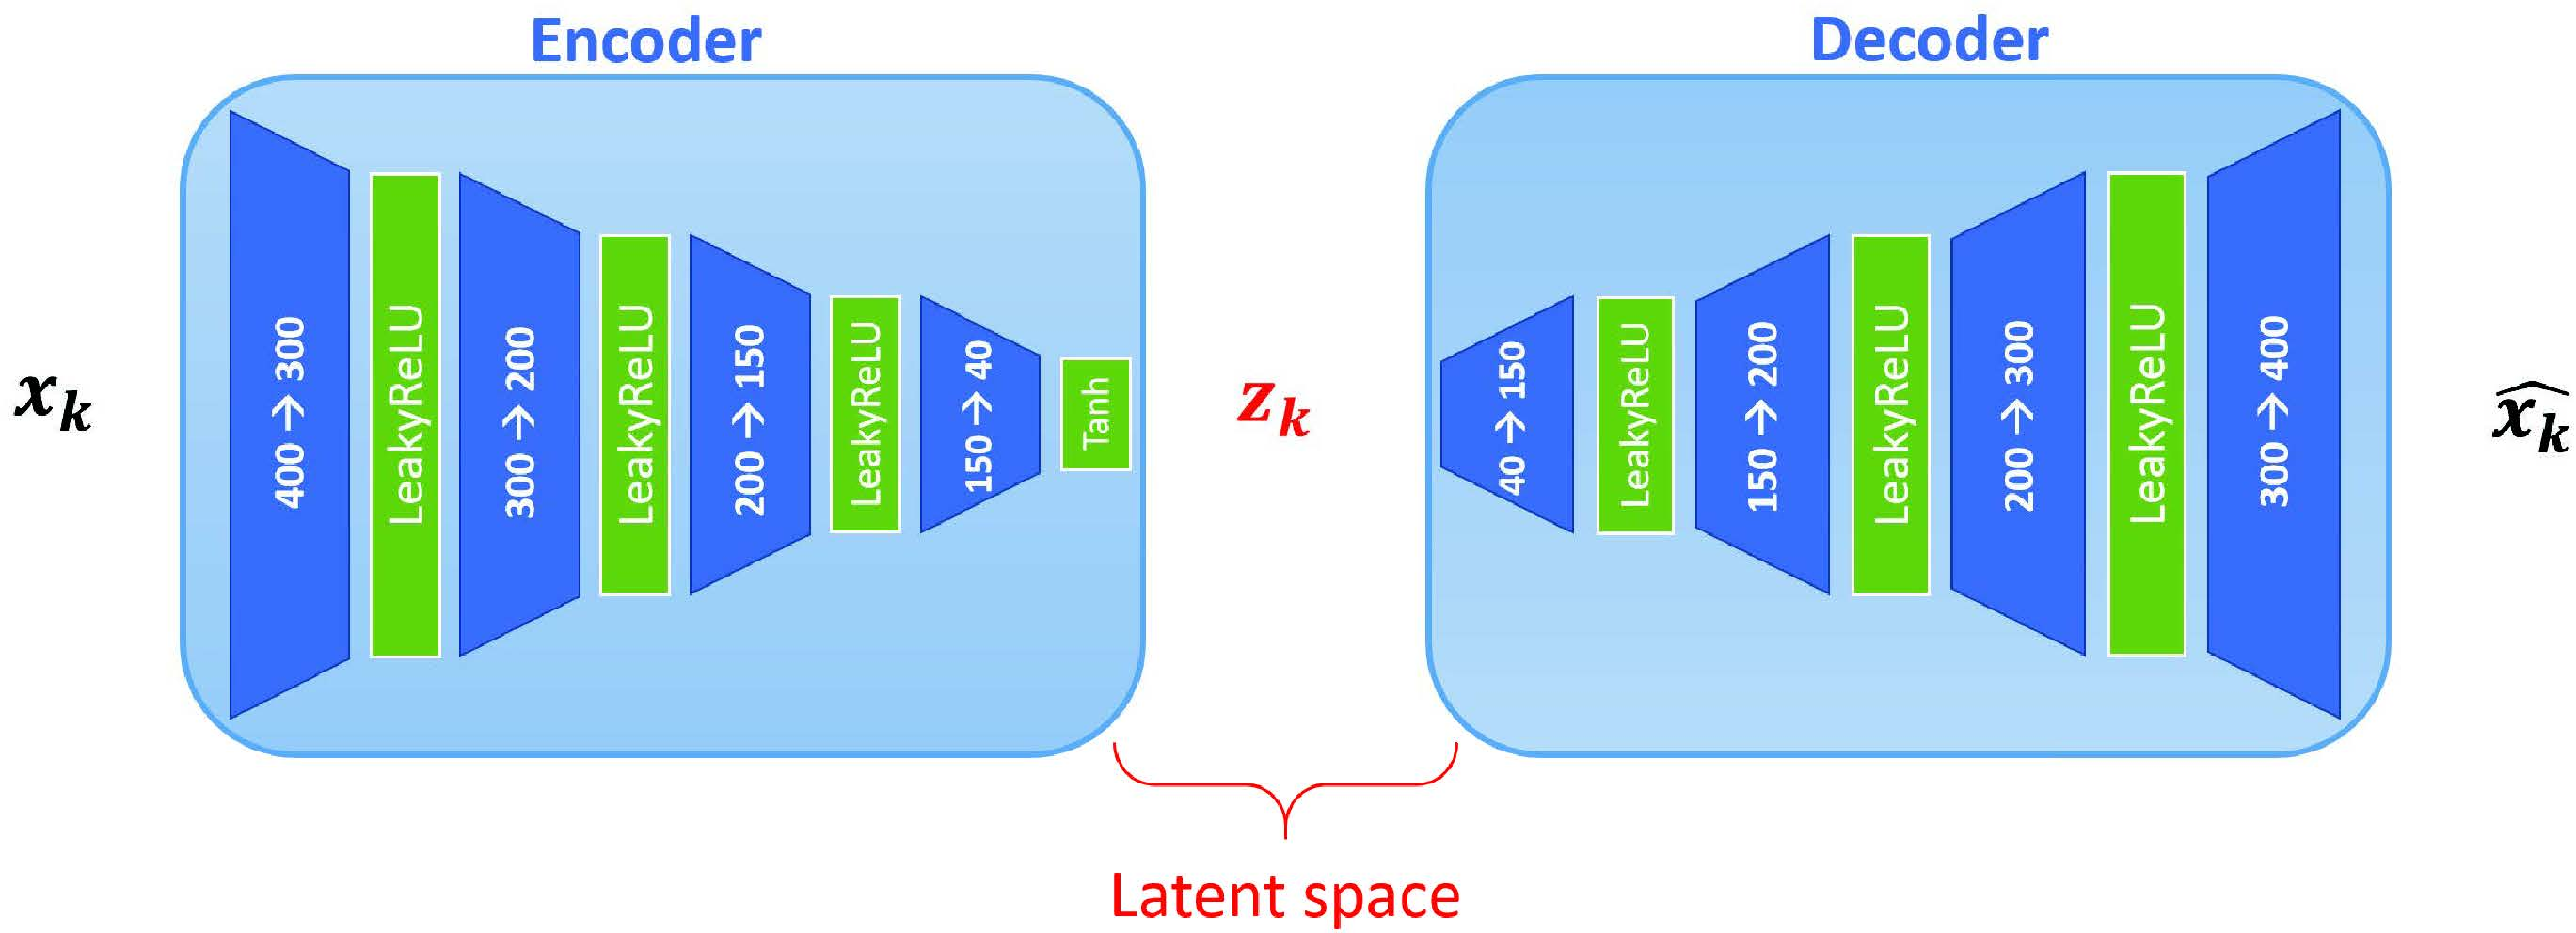
\includegraphics[width=.7\textwidth]{figs/encoder-decoder.jpg}
	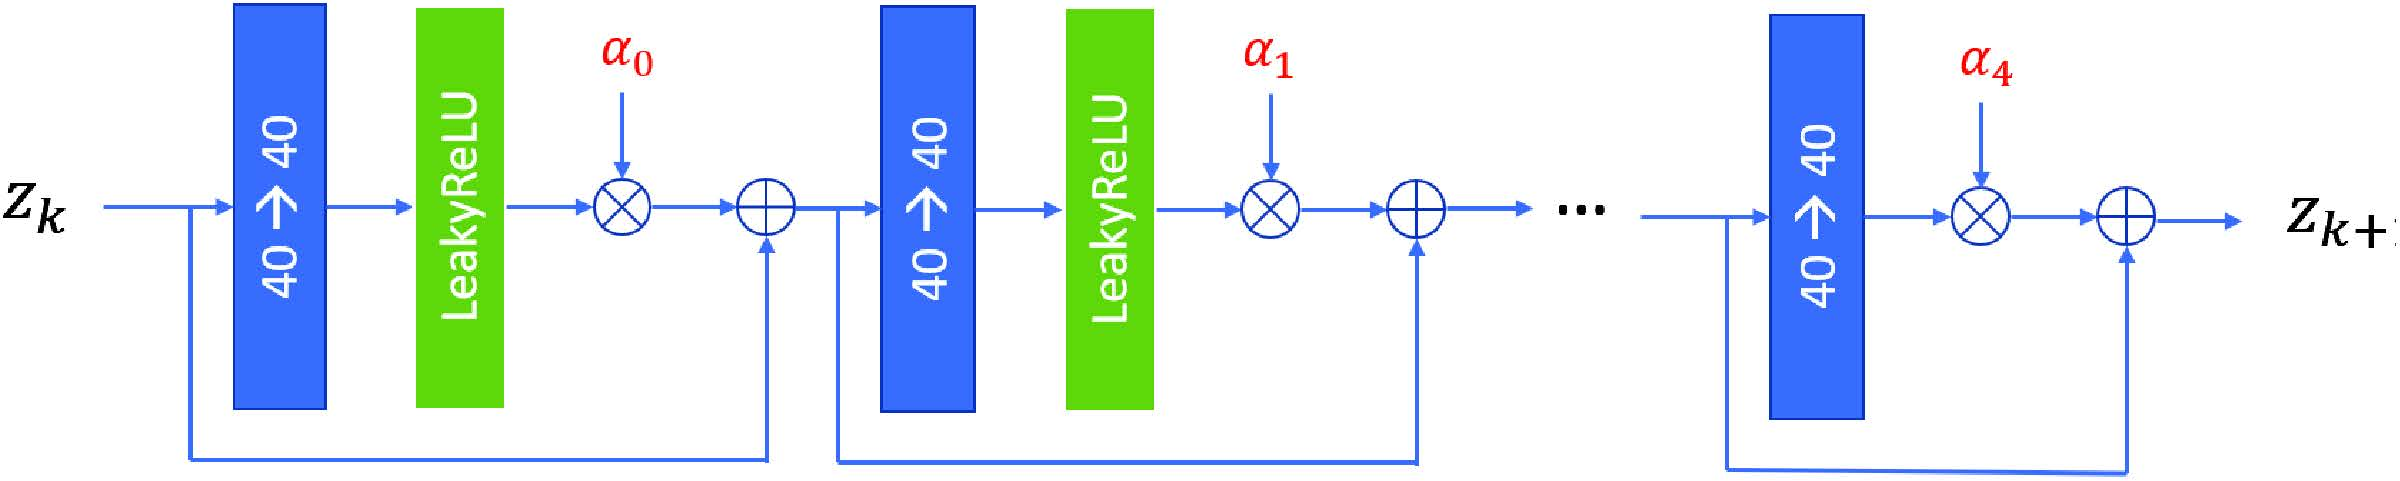
\includegraphics[width=.7\textwidth]{figs/surrogate-model.jpg}
	\caption{The en/decoders consist of fully connected networks, and the surrogate model ultilizes the ReZero structure}
\end{figure}
\subsection{drawbacks}
从实验结果上看,尽管使用神经网络逼近出来的隐空间上的动力学,最终得到的准确度与直接使用RK4数值求解得到的不相上下,且计算速度得到了较大的提升,但结合实际业务需要仍有以下几个难以弥补的问题:
\begin{itemize}
	\item 文章只考虑了一个ODE模型,而实际业务中的模型往往是一个复杂的二维/三维PDE模型,直接使用简单的全连接网络需要的开销极其庞大,且随之带来的是训练难度的增加.
	\item 模型固定在一个规则的网格上,若直接应用到实际场景中,对于非格点上的观测数据,需要使用插值方法将其转化为格点上的数据,这一过程会引入额外的误差.
	\item 对于多模态的数据,例如卫星观测,雷达观测,站点数据等,单一的Encoder-Decoder模型无法直接进行处理.
	\item 若观测场出现数据缺失的情况,需要采取插值等方式对其进行补全,这一操作会影响模型的准确性.
\end{itemize}
\section{Latent Assimilation with Implicit Neural Representations}
\subsection{description}
以$\mR^d$上的动力系统为例,假定我们需要进行同化的物理量为$u:\mR^d\to\mR^c$,其中$d$和$c$分别为物理空间的维数和特征的数目,再设隐空间的维数为$l$,那么普通的Encoder-Decoder模型固定了一个物理空间中的网格$S\subseteq\mR^d$, 使得
\begin{align*}
	\mE & :\mR^{|S|\times c}\to\mR^l,\quad\{u_k(\bm x)\}_{\bm x\in S}\mapsto w_k \\
	\mD & :\mR^l\to\mR^{|S|\times c},\quad w_k\mapsto\{u_k(\bm x)\}_{\bm x\in S}
\end{align*}
满足$\mE$和$\mD$在数据集上接近为一对逆映射.本质上Encoder-Decoder模型寻求的是$\mR^{|S|\times c}$上数据集所在的子流形的某种低维表达.

在本文中,我们提出使用Implicit Neural Representation (INR) 来对物理空间中的数据进行表达,其核心思想是使用一个神经网络$I_\theta:\mR^d\to\mR^c$来逼近$u$,即固定某一个参数化函数空间$\mF=\{I_\theta\mid\theta\in\Theta\}\subseteq\{f\mid\mR^d\to\mR^c\}$,在数据集中训练得到合适的参数$\theta$,使得
\[I_\theta(x)\approx u(x),\,\forall x\in S.\]
由此我们可以建立一个从神经网络参数化表达到物理量分布函数的对应关系:
\begin{align*}
	u      & \mapsto\theta=\argmin_\theta L(I_\theta,u), \\
	\theta & \mapsto I_\theta(\approx u),
\end{align*}
其中$L$刻画了$I_\theta$与实际的物理量$u$之间的差异,可根据实际场景选取不同的定义方式.
\subsection{advantages}
使用INR比起传统的Encoder-Decoder模型有如下几点优势:
\begin{itemize}
	\item 由于INR是一个从物理空间到隐空间的映射,因此可以直接处理非网格化的数据和部分缺测的数据.
	\item INR可以处理多模态的数据,只需要选取适当的criterion $L$,例如
	      \[L(I_\theta,u):=\|\mA(I_\theta)-\mA(u)\|^2\]
	      其中$\mA$可以是某种已知的观测算子,例如卫星观测和雷达观测,故而我们可以同时对卫星资料和雷达资料进行同化.
\end{itemize}
\section{前期实验结果}
\subsection{数据集}
为使数值实验更加贴近真实场景,我们考虑一个二维PDE模型而非原有的Lorenz-96模型,具体来说,我们考虑了2D shallow water equation
\begin{align*}
	\frac{\md u}{\md t} & =-fk\times u-g\nabla h+\nu\Delta u, \\
	\frac{\md h}{\md t} & =-h\nabla\cdot u+\nu\Delta h,
\end{align*}
其中$w=\nabla\times u$.这同时也是开源Python数值模拟库dedalus的样例模型 \url{https://dedalus-project.readthedocs.io/en/latest/pages/examples/ivp_sphere_shallow_water.html},这保证了数据来源的可靠性,初值条件选取为
\[
	u_0=\begin{cases}
		\left(\frac{u_m}{e_n}\exp\left(\frac1{(\phi-\phi_0)(\phi-\phi_1)}\right),0\right), & \phi\in(\phi_0,\phi_1),  \\
		\left(\frac{u_m}{e_n}\exp\left(\frac1{(\phi+\phi_0)(\phi+\phi_1)}\right),0\right), & \phi\in(-\phi_1,\phi_0), \\
		(0,0),                                                                             & \textrm{otherwise},
	\end{cases}
\]
其中$u_m$表示最大速度,取值为$\{60,61,\cdots,80\}$, $\phi_0=\pi/7$, $\phi_1=\pi/2-\phi_0$, $e_n=\exp(-4/(\phi_1-\phi_0)^2)$.$h$的初值涉及求解一个边值问题,具体参数参见\cite{Galewsky-2004}.最终得到1小时为间隔的1000组数据.根据实际效果来看,我们适当截取了第300小时到第700小时的数据,在这一时间段内模型演化的过程较为平稳,且有大量多尺度的特征相互作用.空间方向的网格数我们固定为$128\times64$.
\subsection{baseline}
考虑到参数量的因素,我们放弃将原有的全连接网络直接应用到这一场景中(若直接迁移需要$\mO((2\times128\times64)^2)\sim\mO(2.7\times10^8)$的数据量,且其规模会随实际部署的规模增大而急剧增大),而是考虑使用卷积神经网络来处理这一问题.我们接用了近期在湍流仿真数据压缩领域的SOTA模型AEflow(\url{https://github.com/NREL/AEflow})\cite{AEflow}作为baseline,而隐层的动力学模型仍保留为\cite{Peyron2021LAwithAE}使用的ReZero模型\cite{bachlechner2021rezero}.
\subsection{our model}
我们在INR部分考虑使用DINo模型\cite{yin2023dino},其在encoding部分利用auto-decoding\cite{Park2019Auto-decoding}的思想包含了一个优化内循环,以提高压缩效果\cite{kim2019attentive}.而在representation部分使用了Multiplicative Filter Network\cite{fathony2021multiplicative} with amplitude modulation.

我们在latent dynamics部分直接使用Neural ODE \cite{chen2018neural}的更新算法,以减少模型优化代价,动力学模型则采用了3层全连接结构.
\subsection{实验结果}
\subsubsection{数据压缩和隐空间的动力学}
在对两种网络进行训练后(costs 1.5 RTX3090 $\cdot$ days),我们在测试集上比较两种模型
\begin{itemize}
	\item 数据重构: RMSE($\mD\circ\mE(x),x$);
	\item 预测: RMSE($\mD\circ g\circ\mE(x),x_\textrm{next}$).
\end{itemize}
的精度.
\begin{figure}
	\centering
	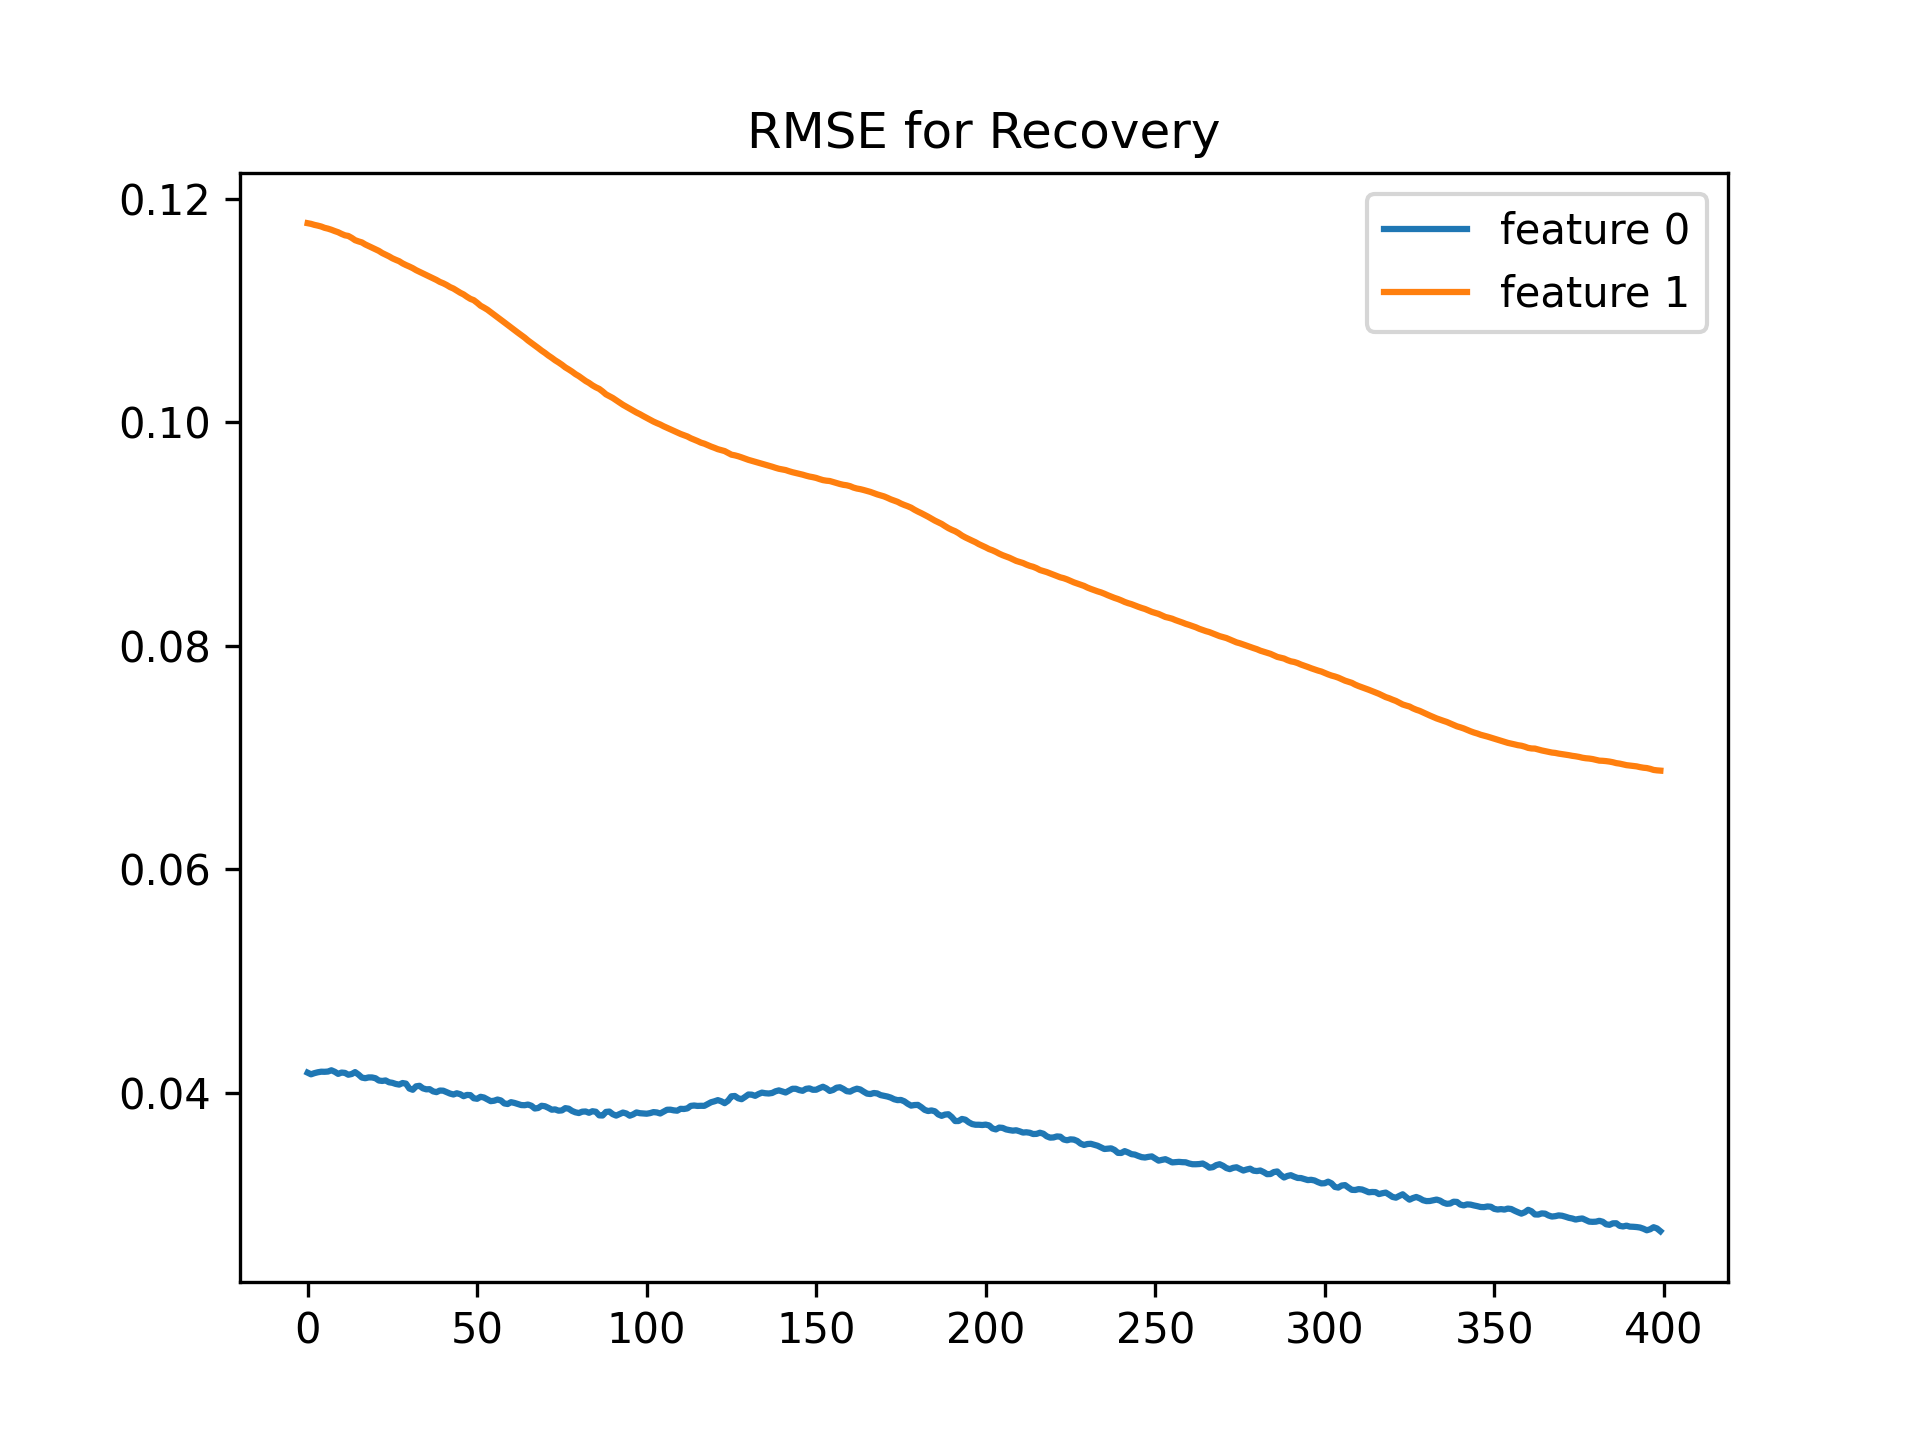
\includegraphics[width=.4\textwidth]{figs/AEflow_main_ae_rmse.png}
	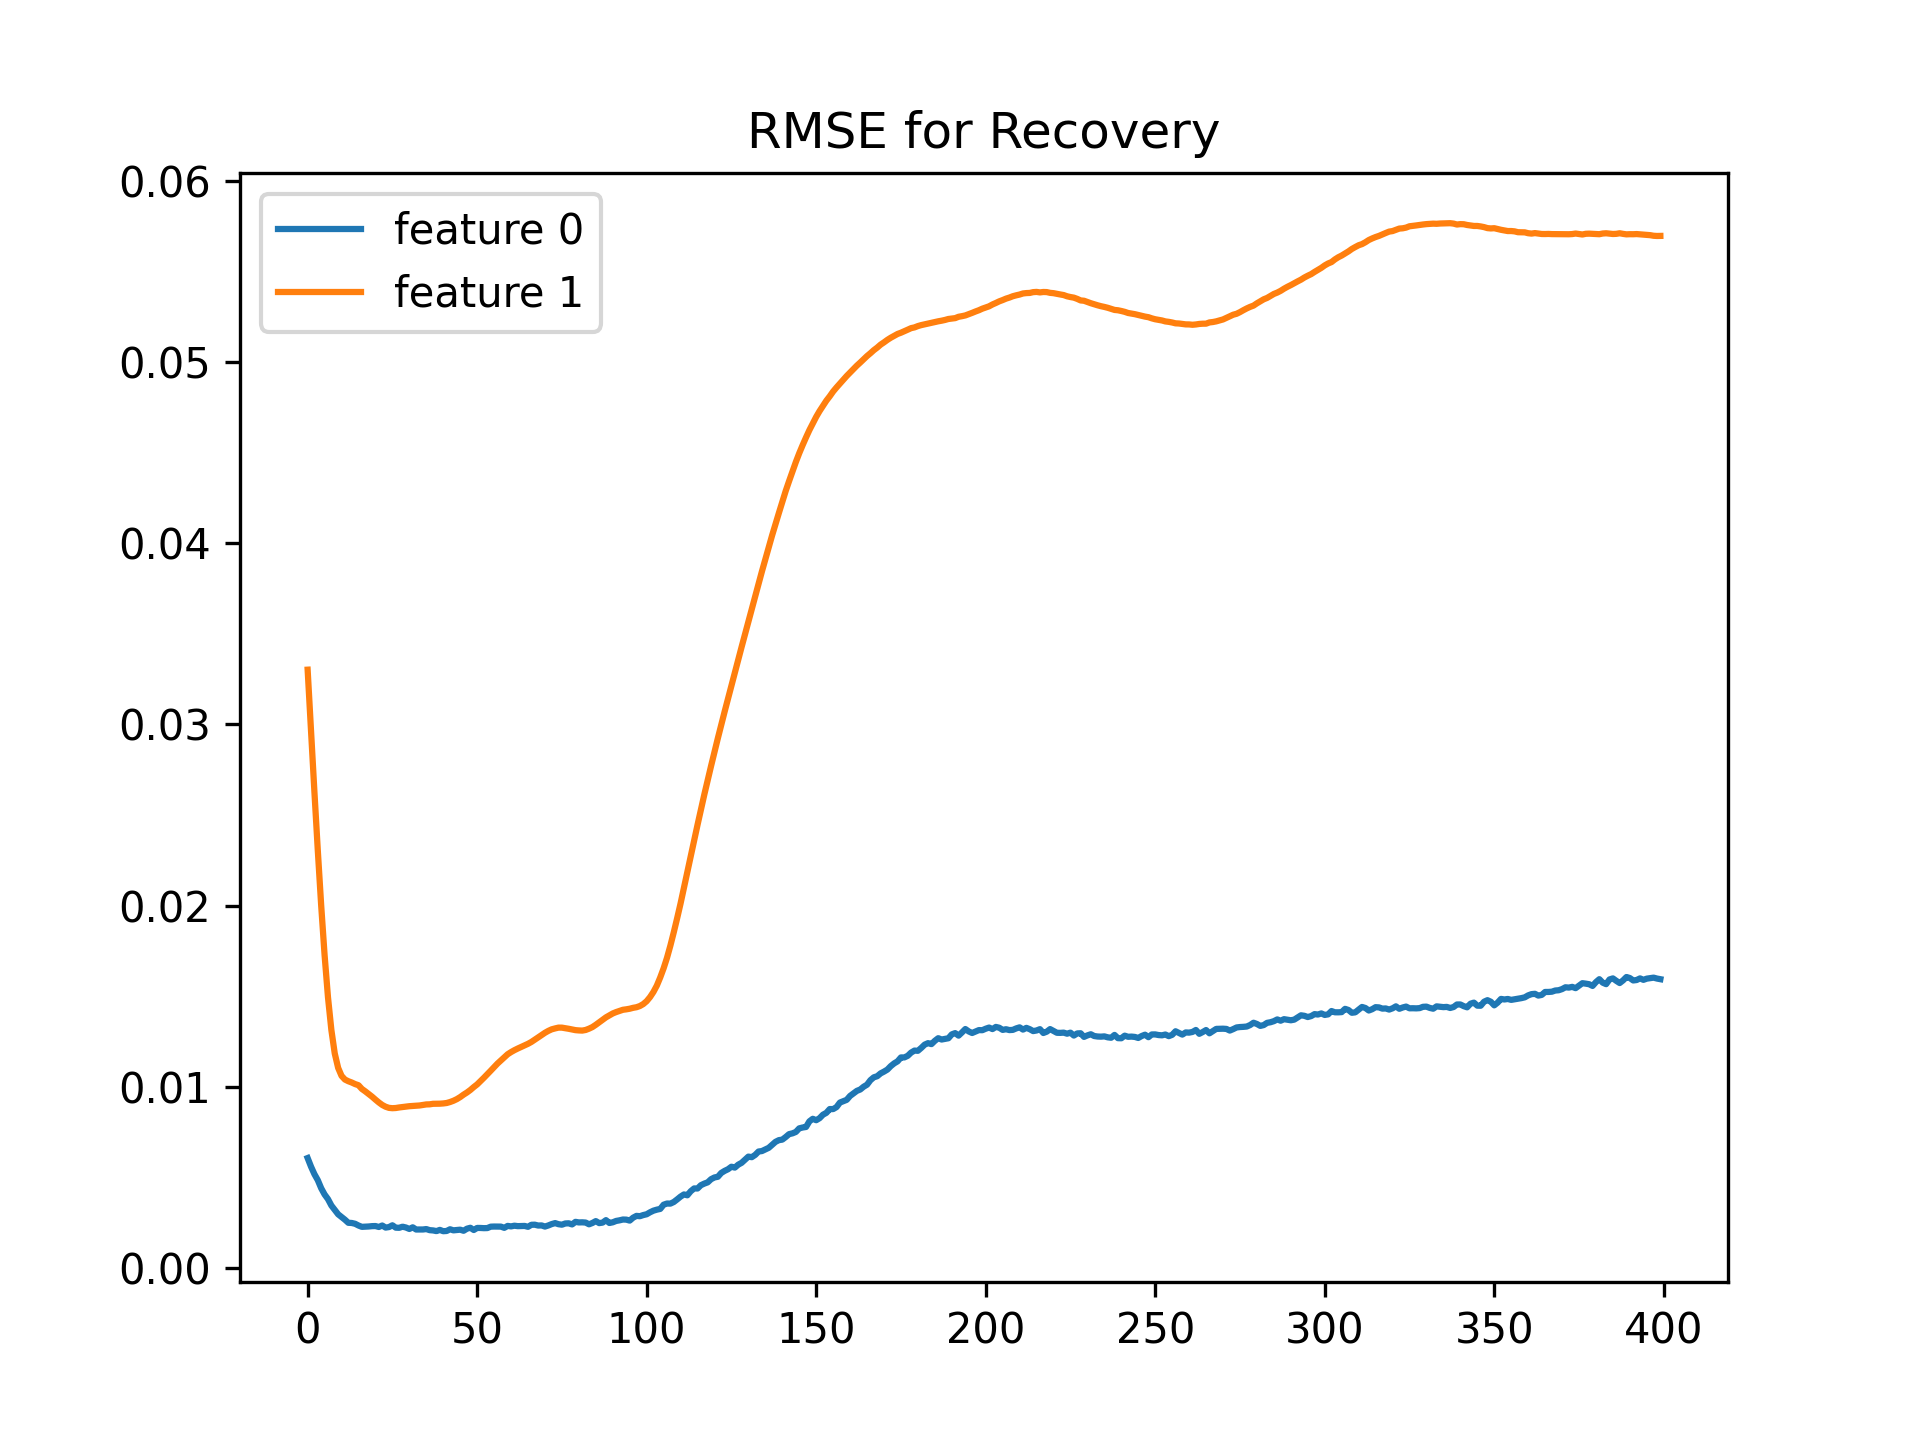
\includegraphics[width=.4\textwidth]{figs/Yin2023LAmain_ae_rmse.png}
	\caption{数据重构(左:AEflow+ReZero;右:Ours)}
\end{figure}
\begin{figure}
	\centering
	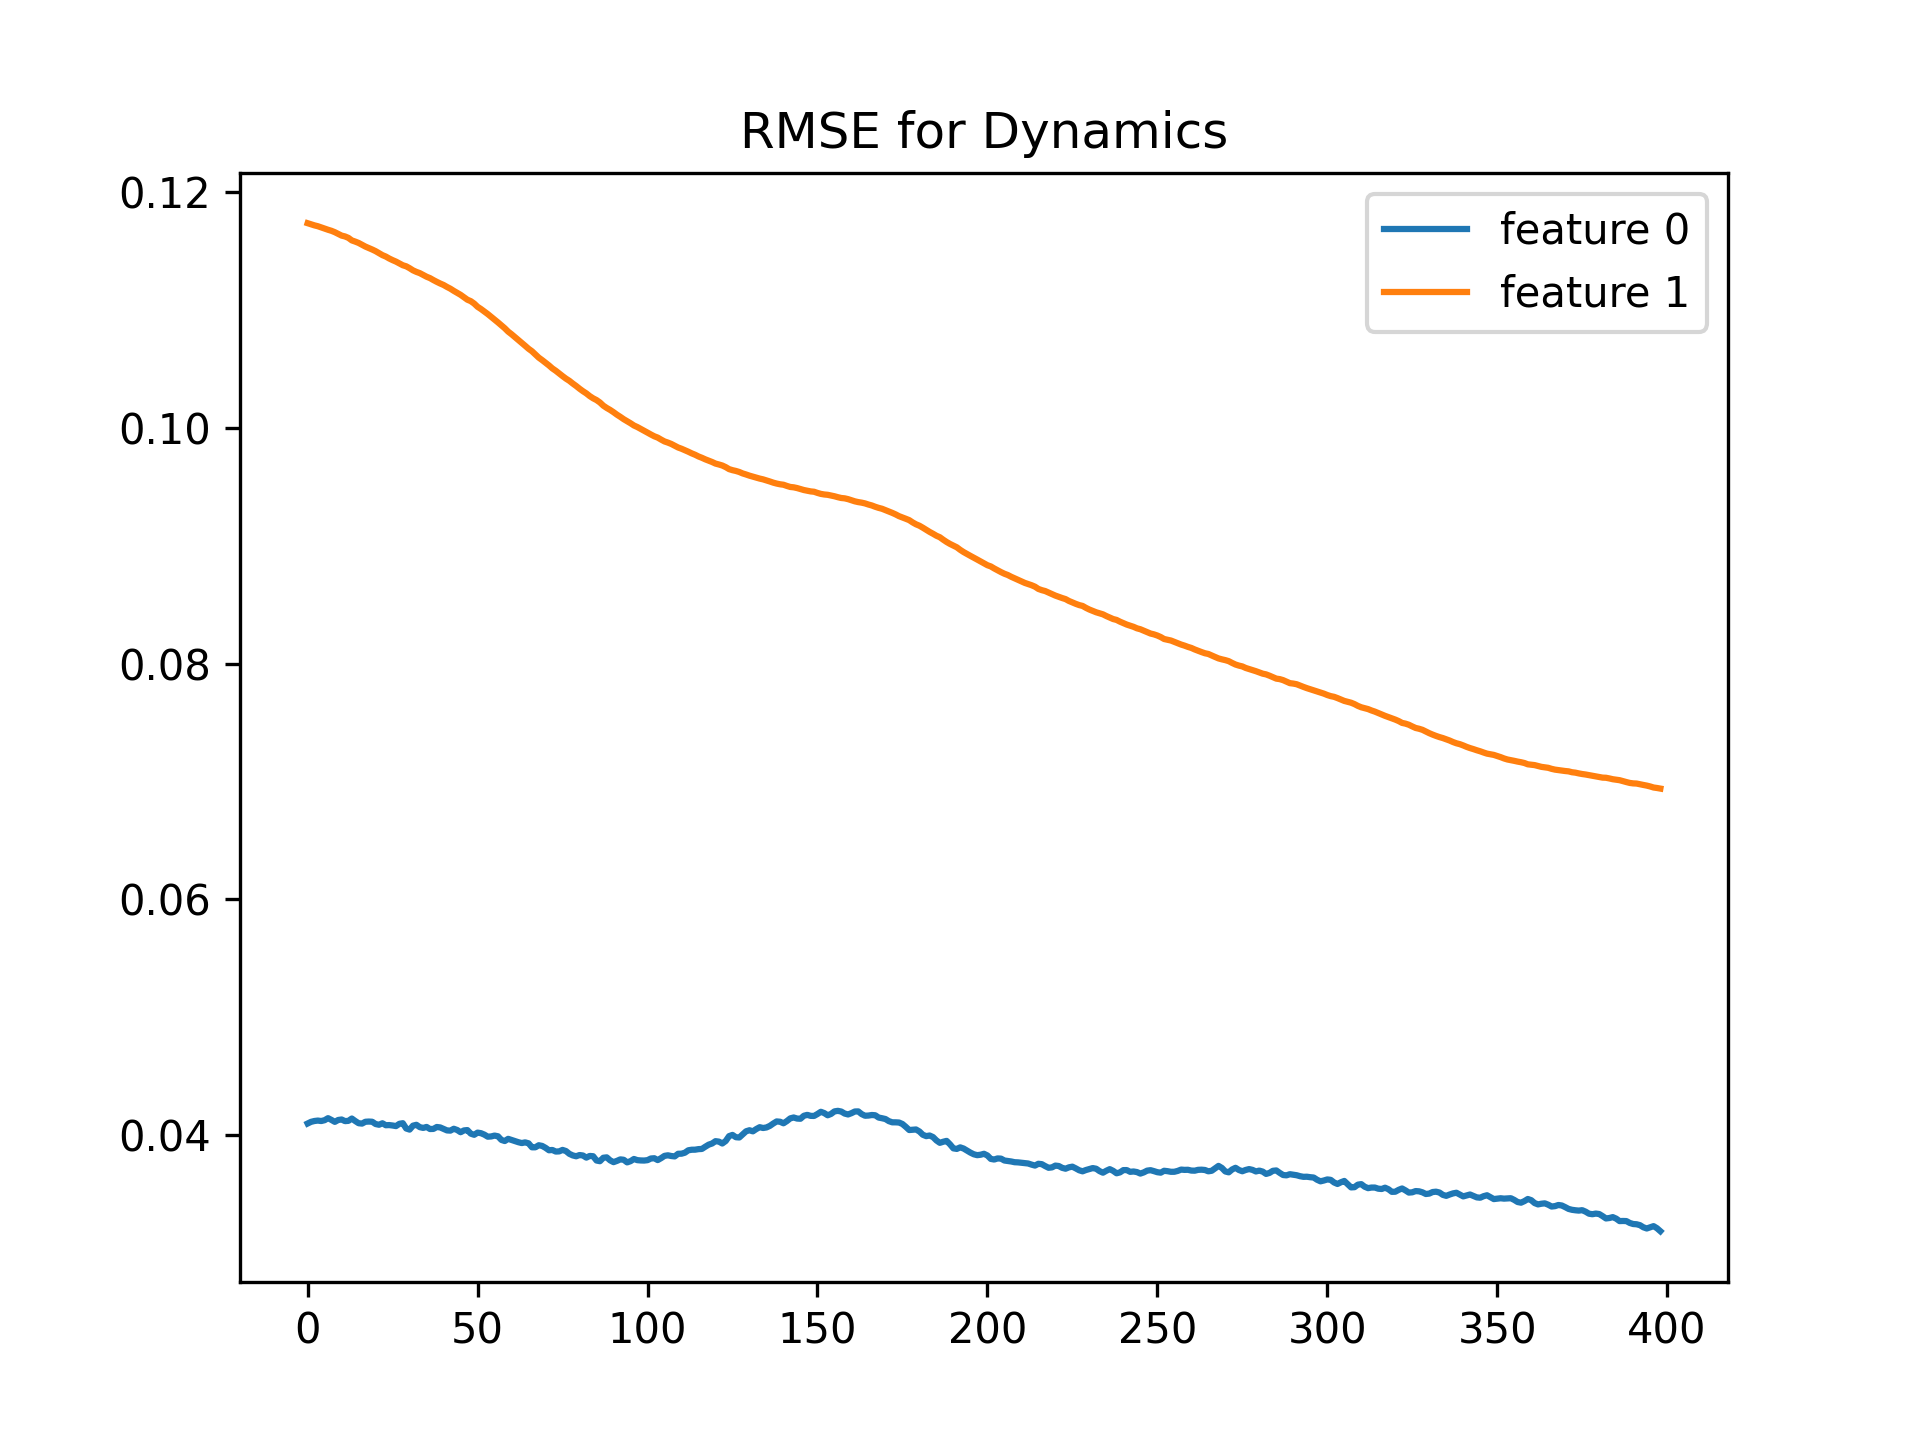
\includegraphics[width=.4\textwidth]{figs/AEflow_main_dyn_rmse.png}
	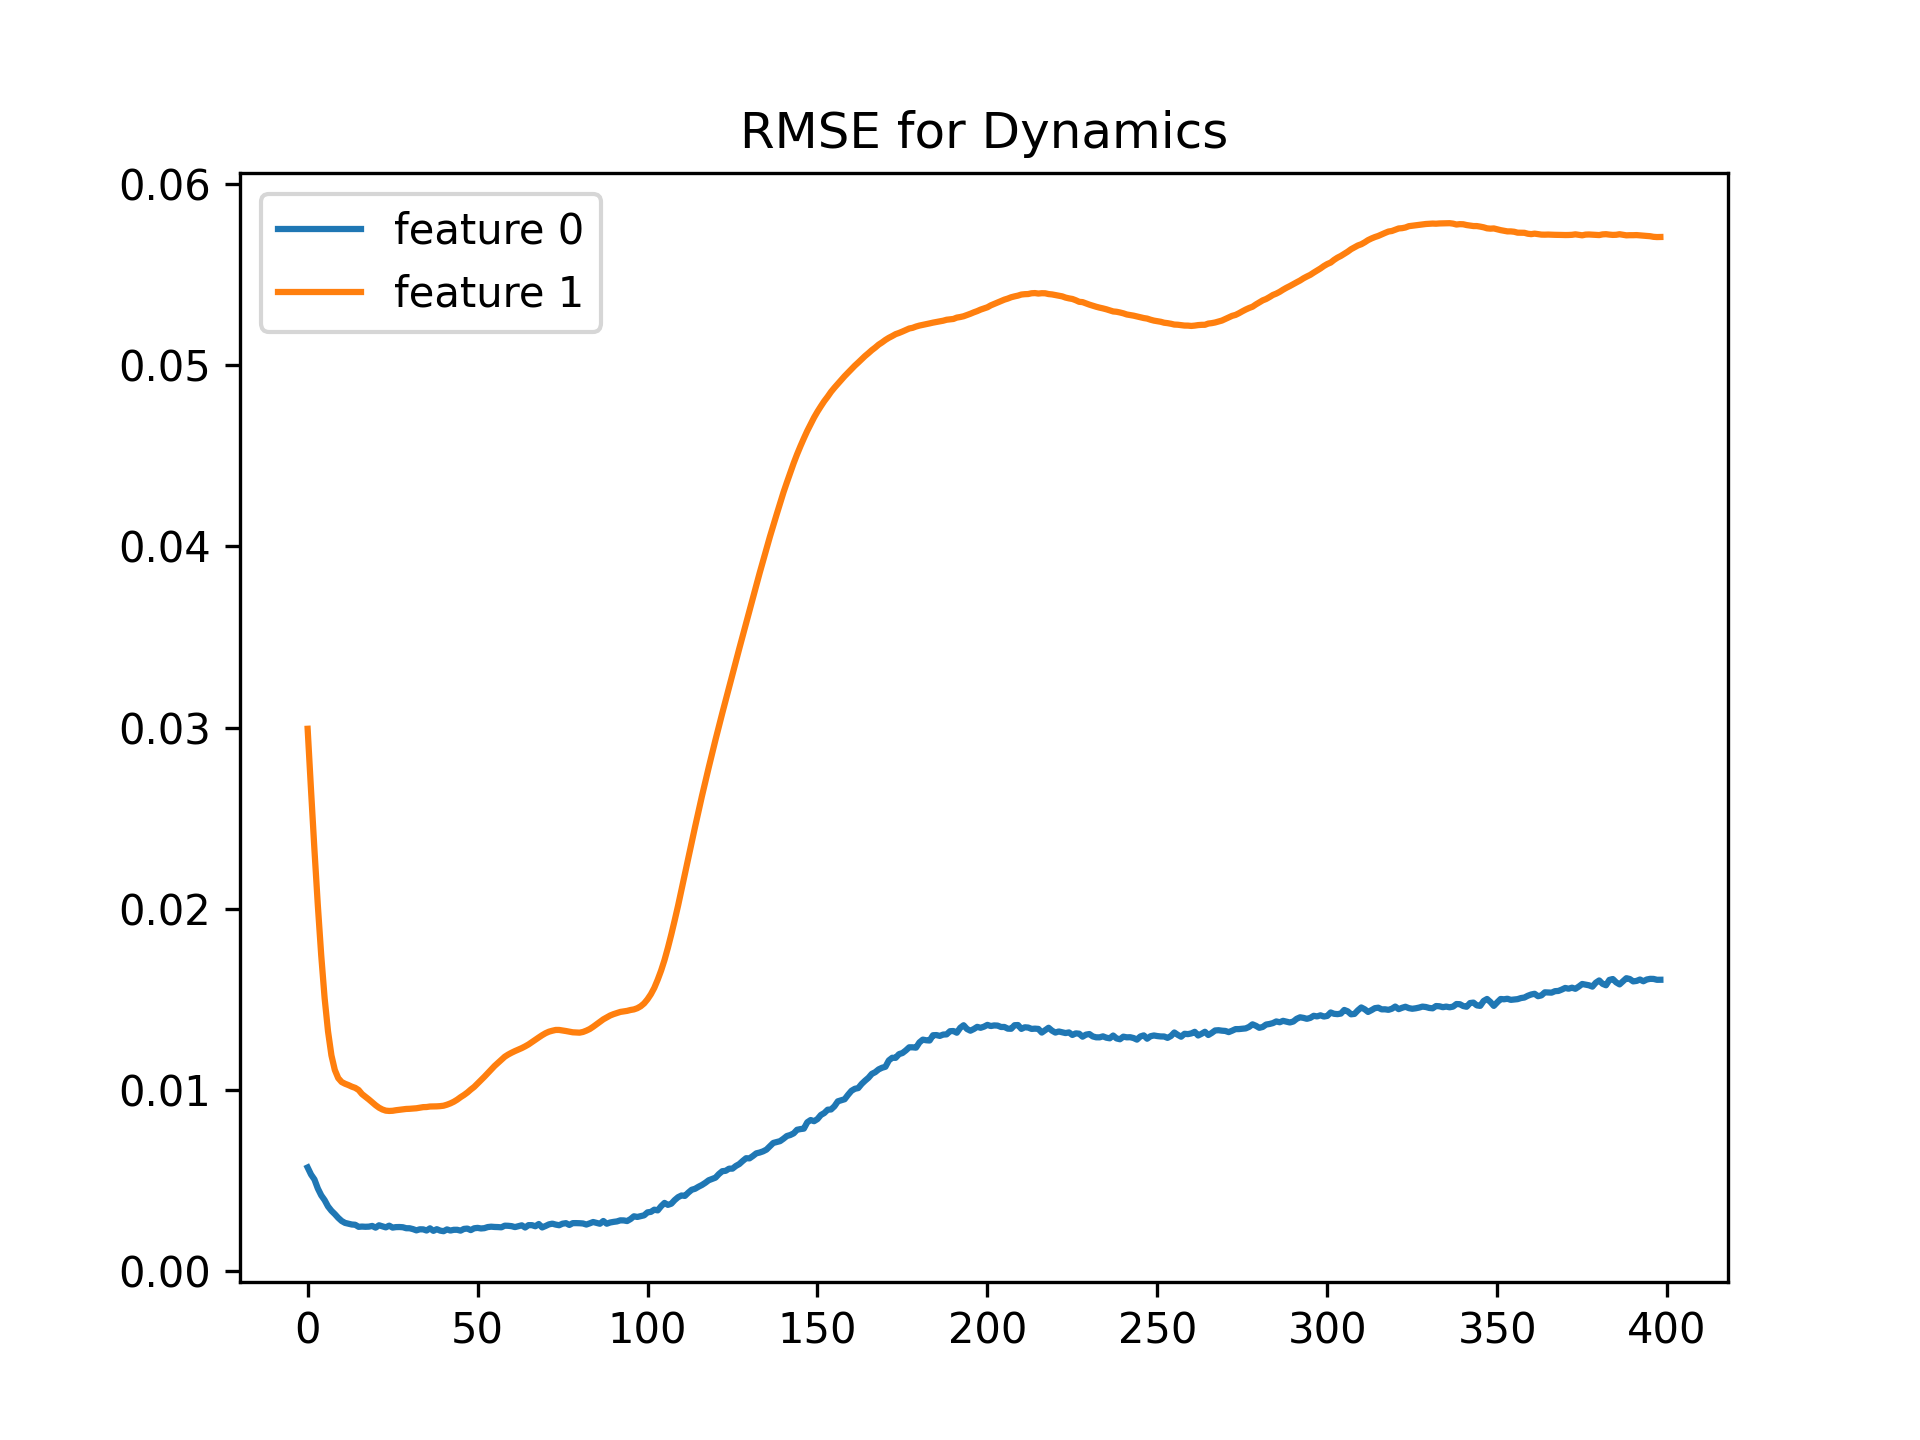
\includegraphics[width=.4\textwidth]{figs/Yin2023LAmain_dyn_rmse.png}
	\caption{数据预测(左:AEflow+ReZero;右:Ours)}
\end{figure}
\subsubsection{latent assimilation}
接下来我们把两种模型应用到不同的同化框架中,并比较其同化效果.我们选取了EnKF, SEnKF, DEnKF, EnSRKF, ETKF, ETKF-Q, 具体算法见附录.观测算子固定为在$128\times64\times2$网格上随机选取\texttt{n\_obs}为 1024, 2048, 4096,分别对应于$1/16=6.25\%$, $1/8=12.5\%$和$1/4=25\%$的观测率.观测误差$\sigma_\textrm{obs}=0.001$.对物理场初值的扰动及隐空间对应的扰动$\sigma$均取0.1.由于目前暂时无法直接刻画我们的替代模型(surrogate model)引入的模型误差,我们对模型误差\texttt{mod\_sigma}取不同的值都进行了实验,得到下表.
\begin{table}[h]
	\centering
	\caption{Comparison of performance metrics for different filters for AEflow-ReZero model.}
	\label{tab:aeflow_comparison}
	\begin{tabular}{c c c c c c c c}
		\hline
		mod\_sigma & $n_{\textrm{obs}}$ & EnKF   & SEnKF  & DEnKF  & EnSRKF & ETKF   & ETKF-Q             \\
		\hline
		1.0        & 1024               & 0.2542 & 0.2734 & 0.2764 & 0.2848 & 0.3351 & 0.1936             \\
		0.5        & 1024               & 0.2468 & 0.2294 & 0.2745 & 0.2626 & 0.2462 & 0.1914             \\
		0.2        & 1024               & 0.2559 & 0.2247 & 0.2255 & 0.2424 & 0.2163 & \underline{0.1766} \\
		0.1        & 1024               & 0.2255 & 0.2283 & 0.2084 & 0.1955 & 0.2123 & 0.2082             \\
		0.05       & 1024               & 0.2490 & 0.2391 & 0.2159 & 0.2067 & 0.2043 & 0.2968             \\
		0.02       & 1024               & 0.2759 & 0.2784 & 0.2698 & 0.2565 & 0.2493 & 0.3906             \\
		0.01       & 1024               & 0.3314 & 0.3746 & 0.3073 & 0.3478 & 0.3114 & 0.4379             \\
		\hline
		1.0        & 2048               & 0.2180 & 0.2159 & 0.2346 & 0.2236 & 0.2281 & \underline{0.1731} \\
		0.5        & 2048               & 0.2085 & 0.1958 & 0.2036 & 0.2003 & 0.1960 & 0.1837             \\
		0.2        & 2048               & 0.2028 & 0.2117 & 0.2023 & 0.2111 & 0.2035 & 0.1978             \\
		0.1        & 2048               & 0.2107 & 0.1997 & 0.2127 & 0.2448 & 0.2129 & 0.1985             \\
		0.05       & 2048               & 0.2338 & 0.2346 & 0.2092 & 0.2396 & 0.2658 & 0.2870             \\
		0.02       & 2048               & 0.2543 & 0.2752 & 0.2369 & 0.2500 & 0.2503 & 0.4051             \\
		0.01       & 2048               & 0.3246 & 0.3513 & 0.2992 & 0.3331 & 0.3156 & 0.4359             \\
		\hline
		1.0        & 4096               & 0.1953 & 0.2105 & 0.2051 & 0.1955 & 0.1963 & \underline{0.1746} \\
		0.5        & 4096               & 0.2035 & 0.1910 & 0.1911 & 0.2019 & 0.2033 & 0.1948             \\
		0.2        & 4096               & 0.1881 & 0.1947 & 0.1941 & 0.1889 & 0.1883 & 0.1905             \\
		0.1        & 4096               & 0.2077 & 0.2025 & 0.1868 & 0.1977 & 0.1966 & 0.2018             \\
		0.05       & 4096               & 0.2138 & 0.2104 & 0.2132 & 0.2004 & 0.2044 & 0.2766             \\
		0.02       & 4096               & 0.2459 & 0.2760 & 0.2277 & 0.2359 & 0.2445 & 0.4026             \\
		0.01       & 4096               & 0.3192 & 0.3583 & 0.2978 & 0.3190 & 0.3141 & 0.4393             \\
		\hline
	\end{tabular}
\end{table}
\begin{table}[h]
	\centering
	\caption{Comparison of performance metrics for different filters for INR-NeuralODE (ours).}
	\label{tab:yin2023_comparison}
	\begin{tabular}{c c c c c c c c}
		\hline
		mod\_sigma & $n_{\textrm{obs}}$ & EnKF   & SEnKF              & DEnKF  & EnSRKF             & ETKF    & ETKF-Q \\
		\hline
		0.1        & 1024               & 0.0619 & 0.0606             & 0.0645 & 0.0585             & nan     & 0.1164 \\
		0.05       & 1024               & 0.0708 & \underline{0.0575} & 0.0598 & 0.0628             & 0.0642  & 0.1290 \\
		0.02       & 1024               & 0.0590 & 0.0598             & 0.0681 & 0.0600             & 0.0615  & 0.1259 \\
		0.01       & 1024               & 0.0578 & 0.0587             & 0.0638 & 0.0581             & 0.0606  & 0.1129 \\
		0.005      & 1024               & 0.0645 & 0.0808             & 0.0686 & 0.0629             & 0.0633  & 0.1098 \\
		0.002      & 1024               & 0.1342 & 0.4105             & 0.0873 & 0.1490             & 0.1147  & 0.1436 \\
		0.001      & 1024               & 4.3256 & 1.5767             & 5.8916 & 2.9570             & 29.9085 & 0.4060 \\
		\hline
		0.1        & 2048               & 0.0454 & 0.0465             & 0.0498 & 0.0454             & nan     & 0.1252 \\
		0.05       & 2048               & 0.0442 & 0.0440             & 0.0466 & 0.0439             & 0.0445  & 0.1108 \\
		0.02       & 2048               & 0.0443 & \underline{0.0437} & 0.0463 & 0.0445             & 0.0443  & 0.1156 \\
		0.01       & 2048               & 0.0459 & 0.0449             & 0.0466 & 0.0445             & 0.0448  & 0.1275 \\
		0.005      & 2048               & 0.0518 & 0.0544             & 0.0496 & 0.0505             & 0.0501  & 0.1141 \\
		0.002      & 2048               & 0.0656 & 0.0802             & 0.0623 & 0.0751             & 0.0765  & 0.1337 \\
		0.001      & 2048               & 0.3156 & 1.0958             & 0.1431 & 0.2924             & 0.1659  & 0.1936 \\
		\hline
		0.1        & 4096               & 0.0412 & 0.0414             & 0.0433 & 0.0418             & nan     & 0.1413 \\
		0.05       & 4096               & 0.0411 & 0.0405             & 0.0420 & \underline{0.0400} & nan     & 0.1231 \\
		0.02       & 4096               & 0.0417 & 0.0420             & 0.0438 & 0.0412             & 0.0413  & 0.1145 \\
		0.01       & 4096               & 0.0416 & 0.0421             & 0.0424 & 0.0417             & 0.0416  & 0.1144 \\
		0.005      & 4096               & 0.0448 & 0.0530             & 0.0482 & 0.0467             & 0.0468  & 0.1074 \\
		0.002      & 4096               & 0.0694 & 0.1119             & 0.0637 & 0.0679             & 0.0731  & 0.1269 \\
		0.001      & 4096               & 0.1392 & 0.4200             & 0.1451 & 0.2540             & 0.2150  & 0.2179 \\
		\hline
	\end{tabular}
\end{table}

对两种模型分别选取表现较好的一组参数,绘制出同化准确度随时间的变化关系如图所示.
\begin{figure}
	\centering
	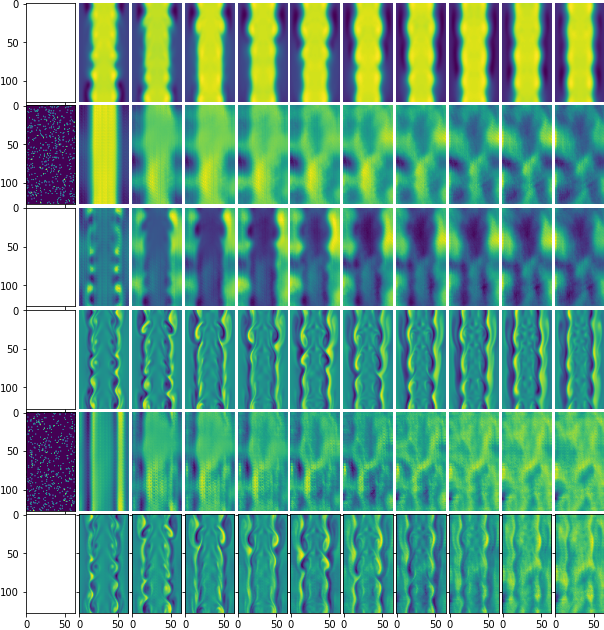
\includegraphics[width=.8\textwidth]{figs/sigma_x_b=0.1_sigma_z_b=0.1_mod_sigma=0.1_n_obs=1024_method=ETKF-Q_plot.png}
	\caption{AEflow+ReZero+ETKF-Q, mod\_sigma=0.1, $n_\textrm{obs}=1024$.前三行对应feature 0,后三行对应feature 1,其中对于每个feature第一行是真实值,第二行第一个是观测位置,紧接着的是同化结果(每个40小时取一个frame),第三行是误差.}
\end{figure}
\begin{figure}
	\centering
	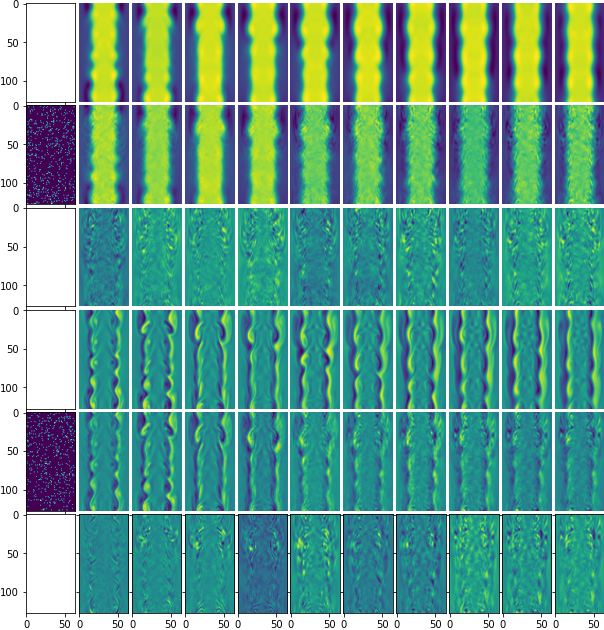
\includegraphics[width=.8\textwidth]{figs/sigma_x_b=0.1_sigma_z_b=0.1_mod_sigma=0.05_n_obs=1024_method=SEnKF_plot.png}
	\caption{Our model+SEnKF, mod\_sigma=0.05, $n_\textrm{obs}=1024$.前三行对应feature 0,后三行对应feature 1,其中对于每个feature第一行是真实值,第二行第一个是观测位置,紧接着的是同化结果(每个40小时取一个frame),第三行是误差.}
\end{figure}
\begin{figure}
	\centering
	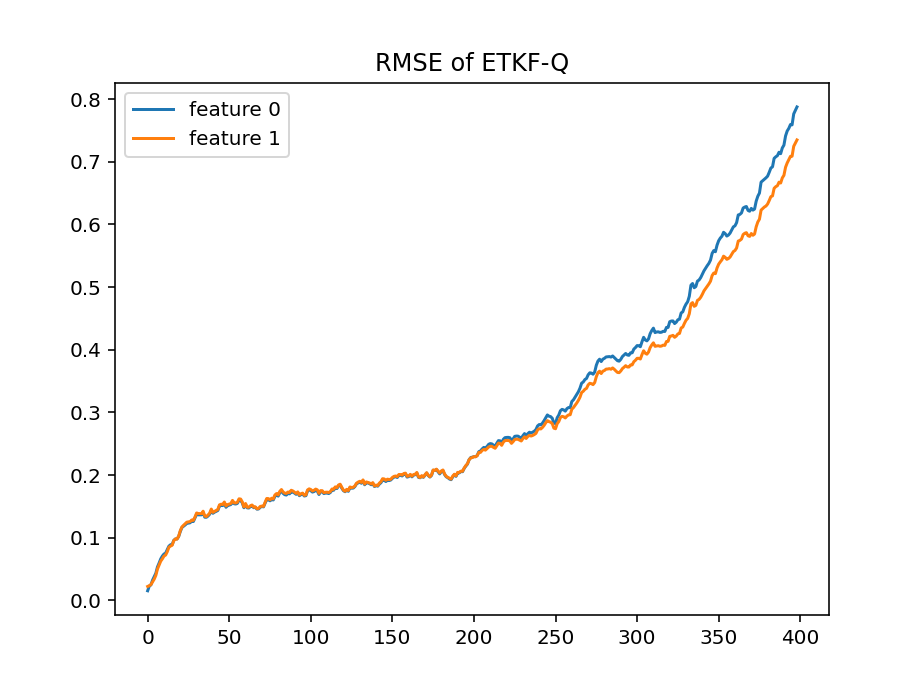
\includegraphics[width=.4\textwidth]{figs/sigma_x_b=0.1_sigma_z_b=0.1_mod_sigma=0.1_n_obs=1024_method=ETKF-Q_rmse.png}
	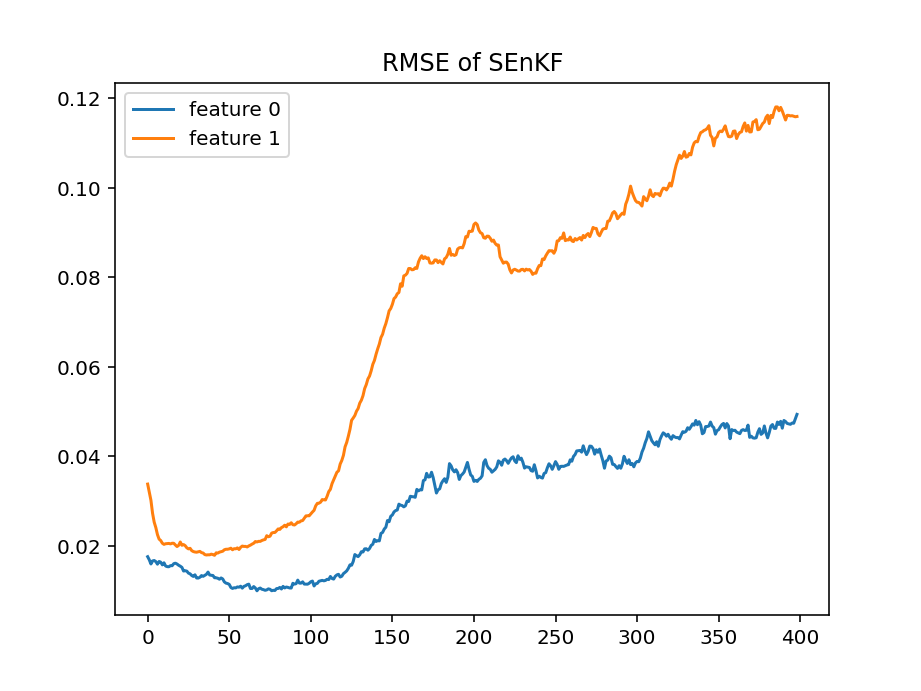
\includegraphics[width=.4\textwidth]{figs/sigma_x_b=0.1_sigma_z_b=0.1_mod_sigma=0.05_n_obs=1024_method=SEnKF_rmse.png}
	\caption{同化误差随时间的变化关系(左:AEflow+ReZero+ETKF-Q, mod\_sigma=0.1, $n_\textrm{obs}=1024$;右:Our model+SEnKF, mod\_sigma=0.05, $n_\textrm{obs}=1024$)}
\end{figure}
\subsubsection{结果分析}
相较于Encoder-Decoder模型(AEflow+ReZero),我们的模型除了前述INR自身的优点以外有如下优势:
\begin{itemize}
	\item 数据重构和预测的精度高于AEflow+ReZero(约0.5到1个数量级);
	\item 结合传统同化方法时,同化误差随时间的变化更加平稳,同化误差更小(约0.5到1个数量级),且未出现发散的现象;
	\item 观察同化的结果图可知,我们的模型能够更好地保留物理场的结构信息,在长期运行中保持相对稳定.
\end{itemize}
\section{未来工作}
虽然我们的模型相对于已有模型存在明显提升,泛用性也更强,但仍有以下问题有待解决:
\begin{itemize}
	\item 选择的数值模型结构较为简单,若能运用在QG equation或者真实数据(如ERA5)上将有更强的说服力;
	\item 训练数据集的选取以及训练算法仍有待改进,从测试结果可以看出我们的模型在时次靠后的数据上表现较差;
	\item 模型本身的创新性不强,现仅利用已有的模型进行拼凑,未来可以考虑针对同化这一具体场景设计更加合理的模型结构,如适当地考虑数据本身具有的噪声,利用Bayesian neural network\cite{Goan2020BNNsurvey}等框架设计具体的结构.
	\item latent dynamics can be replaced with stochastic dynamics (Neural SDE) so that adapted model errors can be fed to DA frameworks.
	\item more dedicate structures for the INR can be used to handle the multi-scale features in the system.
\end{itemize}
\bibliographystyle{plain} % We choose the "plain" reference style
\bibliography{20230512summary} % Entries are in the refs.bib file
\appendix
\section{同化算法}
\subsection{EnKF}
ref:
Long short-term memory embedded
nudging schemes for nonlinear data
assimilation of geophysical flows. Pawar et al. doi: 10.1063/5.0012853

\subsubsection{Forecast step}
\begin{itemize}
	\item Forward propagation:
	      $$
		      x_k^{b,j}=\mathcal{M}_k(x_{k-1}^{a,j})+\varepsilon_k^{M,j},\quad \varepsilon_k^{M,j}\sim\mathcal{N}(0,\Sigma_k^M);
	      $$
	      perturbed propagation

\end{itemize}
\subsubsection{Analysis step}
\begin{itemize}
	\item Obtain the ensemble mean and anomaly matrix from the ensembles:
	      \begin{align*}
		      x_k^b & = \frac1N\sum_{j=1}^Nx_k^{b,j},                                           \\
		      X_k^b & = \frac1{\sqrt{N-1}}(x_k^{b,j} - x_k^b)_{j=1}^N\in\mathbb{R}^{n\times N}, \\
		      P_k^b & = X_k^bX_k^{bT}
	      \end{align*}
	\item Obtain the perturbed observation vectors:
	      $$
		      z_k^{o,j} = y_k^o + \varepsilon_k^{o,j},\quad\varepsilon_k^{o,j}\sim\mathcal{N}(0,\Sigma_k^o);
	      $$
	\item Innovation vectors
	      $$
		      d_k^j = z_k^{o,j} - \mathcal{H}_k(x_k^{b,j});
	      $$
	\item Evaluate the Kalman gain matrix
	      \begin{align*}
		      K_k & = P_k^bH_k^T(H_kP_k^bH_k^T+\Sigma_k^o)^{-1}                 \\
		          & = X_k^bX_k^{bT}H_k^T(H_kX_k^bX_k^{bT}H_k^T+\Sigma_k^o)^{-1} \\
		          & = P_{xz}(P_{zz}+\Sigma_k^o)^{-1},
	      \end{align*}
	      where
	      $$
		      P_{xz} = X_k^b(H_kX_k^b)^T,\quad P_{zz} = (H_kX_k^b)(H_kX_k^b)^T.
	      $$
	\item Update the analyzed ensembles:
	      $$
		      x_k^{a,j}=x_k^{b,j}+K_kd_k^j.
	      $$
\end{itemize}
\subsection{SEnKF}
ref:
Data assimilation: Methods, Algorithms and Applications. Bocquet

(https://epubs.siam.org/doi/epdf/10.1137/1.9781611974546.ch6)

\subsubsection{Forecast step}
\begin{itemize}
	\item Forward propagation:
	      $$
		      x_k^{b,j}=\mathcal{M}_k(x_{k-1}^{a,j})+\varepsilon_k^{M,j},\quad \varepsilon_k^{M,j}\sim\mathcal{N}(0,\Sigma_k^M);
	      $$
	      perturbed propagation
\end{itemize}


\subsubsection{Analysis step}
\begin{itemize}
	\item Obtain the ensemble mean and anomaly matrix from the ensembles:
	      \begin{align*}
		      x_k^b & = \frac1N\sum_{j=1}^Nx_k^{b,j},                                           \\
		      X_k^b & = \frac1{\sqrt{N-1}}(x_k^{b,j} - x_k^b)_{j=1}^N\in\mathbb{R}^{n\times N}, \\
		      P_k^b & = X_k^bX_k^{bT}
	      \end{align*}
	\item Obtain the perturbed observation vectors:
	      $$
		      z_k^{o,j} = y_k^o + \varepsilon_k^{o,j},\quad\varepsilon_k^{o,j}\sim\mathcal{N}(0,\Sigma_k^o);
	      $$
	\item Compute the ensemble means and the normalized anomalies for the perturbed background estimates for the observations:
	      \begin{align*}
		      y_k^{p,j} & = \mathcal{H}_k(x_k^{b,j}) - \varepsilon_k^{o,j}                          \\
		      y_k^p     & = \frac1N\sum_{j=1}^Ny_k^{p,j},                                           \\
		      Y_k^p     & = \frac1{\sqrt{N-1}}(y_k^{p,j} - y_k^p)_{j=1}^N\in\mathbb{R}^{n\times N}.
	      \end{align*}
	\item Kalman gain matrix
	      $$
		      K_k=X_k^bY_k^{pT}(Y_k^pY_k^{pT})^{-1}
	      $$
	\item Update the analyzed ensembles:
	      $$
		      x_k^{a,j}=x_k^{b,j}+K_k(z_k^{o,j}-\mathcal{H}_k(x_k^{b,j})).
	      $$
\end{itemize}
\subsection{DEnKF}
ref:
Data assimilation: Methods, Algorithms and Applications. Bocquet

(https://epubs.siam.org/doi/epdf/10.1137/1.9781611974546.ch6)

\subsubsection{Forecast step}
\begin{itemize}
	\item Forward propagation:
	      $$
		      x_k^{b,j}=\mathcal{M}_k(x_{k-1}^{a,j})+\varepsilon_k^{M,j},\quad \varepsilon_k^{M,j}\sim\mathcal{N}(0,\Sigma_k^M);
	      $$
	      perturbed propagation
\end{itemize}

\subsubsection{Analysis step}
\begin{itemize}
	\item Obtain the ensemble mean and anomaly matrix from the ensembles:
	      \begin{align*}
		      x_k^b & = \frac1N\sum_{j=1}^Nx_k^{b,j},                                           \\
		      X_k^b & = \frac1{\sqrt{N-1}}(x_k^{b,j} - x_k^b)_{j=1}^N\in\mathbb{R}^{n\times N}, \\
		      P_k^b & = X_k^bX_k^{bT}
	      \end{align*}
	\item Innovation vectors
	      $$
		      d_k = y_k^o - \mathcal{H}_k(x_k^b);
	      $$
	\item Kalman gain matrix
	      \begin{align*}
		      K_k & = P_k^bH_k^T(H_kP_k^bH_k^T+\Sigma_k^o)^{-1}                 \\
		          & = X_k^bX_k^{bT}H_k^T(H_kX_k^bX_k^{bT}H_k^T+\Sigma_k^o)^{-1} \\
		          & = P_{xz}(P_{zz}+\Sigma_k^o)^{-1},
	      \end{align*}
	\item Assimilate the forecast state estimate with the observation
	      $$
		      x_k^a = x_k^b + K_k(y_k^o - \mathcal{H}_k(x_k^b))
	      $$
	\item Compute the analyzed anomalies
	      $$
		      X_k^a = X_k-\frac12K_kH_kX_k
	      $$
	\item Compute the analyzed ensembles
	      $$
		      x_k^{a,j} = \sqrt{N-1}X_k^a[:, j] + x_k^a
	      $$
\end{itemize}
\subsection{EnSRKF}
ref:
Data assimilation: Methods, Algorithms and Applications. Bocquet

(https://epubs.siam.org/doi/epdf/10.1137/1.9781611974546.ch6)

\subsubsection{Forecast step}
\begin{itemize}
	\item Forward propagation:
	      $$
		      x_k^{b,j}=\mathcal{M}_k(x_{k-1}^{a,j})+\varepsilon_k^{M,j},\quad \varepsilon_k^{M,j}\sim\mathcal{N}(0,\Sigma_k^M);
	      $$
	      perturbed propagation
\end{itemize}

\subsubsection{Analysis step}
\begin{itemize}
	\item Obtain the ensemble mean and anomaly matrix from the ensembles:
	      \begin{align*}
		      x_k^b & = \frac1N\sum_{j=1}^Nx_k^{b,j},                                           \\
		      X_k^b & = \frac1{\sqrt{N-1}}(x_k^{b,j} - x_k^b)_{j=1}^N\in\mathbb{R}^{n\times N}, \\
		      P_k^b & = X_k^bX_k^{bT}
	      \end{align*}
	\item Compute the ensemble means and the normalized anomalies for the observations:
	      \begin{align*}
		      y_k^{b,j} & = \mathcal{H}_k(x_k^{b,j})                                                \\
		      y_k^b     & = \frac1N\sum_{j=1}^Ny_k^{b,j},                                           \\
		      Y_k^b     & = \frac1{\sqrt{N-1}}(y_k^{b,j} - y_k^b)_{j=1}^N\in\mathbb{R}^{m\times N};
	      \end{align*}
	\item Transforming matrix
	      $$
		      T_k = (I_m+Y_k^{bT}(\Sigma_k^o)^{-1}Y_k^b)^{-1} = (I_m + S_k^TS_k)^{-1}
	      $$
	      for $S_k=(\Sigma_k^o)^{-1/2}Y_k^b$;

	\item normalized innovation vector
	      $$
		      \delta_k = (\Sigma_k^o)^{-1/2}(y_k^o-y_k^b)
	      $$
	\item Evaluate the original Kalman gain matrix
	      \begin{align*}
		      K_k & = P_k^bH_k^T(H_kP_k^bH_k^T+\Sigma_k^o)^{-1}                 \\
		          & = X_k^bX_k^{bT}H_k^T(H_kX_k^bX_k^{bT}H_k^T+\Sigma_k^o)^{-1} \\
		          & = P_{xz}(P_{zz}+\Sigma_k^o)^{-1},
	      \end{align*}
	      where
	      $$
		      P_{xz} = X_k^b(H_kX_k^b)^T,\quad P_{zz} = (H_kX_k^b)(H_kX_k^b)^T.
	      $$
	\item Obtain the modified Kalman gain matrix
	      $$
		      \tilde K = K(I + (I + H_kP_k^bH_k^T(\Sigma_k^o)^{-1})^{-1/2})^{-1}
	      $$
	\item Update the analyzed ensembles
	      \begin{align*}
		      w_k^a     & = (I_m + Y_k^{bT}\Sigma_k^o Y_b)^{-1}Y^{bT}(\Sigma_k^o)^{-1}(y_k^o-y_k^b)=T_kS_k^T\delta_k \\
		      x_k^a     & = x_k^b + X_k^bw_k^a = x_k^b + X_k^bT_kS_k^T\delta_k                                       \\
		      X_k^a     & = (I_n - \tilde{K}_kH_k)X_k^bU,\, U1=1, U\in O(N)                                          \\
		      x_k^{a,j} & = x_k^a + \sqrt{N-1}X_k^a[:, j]
	      \end{align*}
	      OR:
	      $$
		      (x_k^{a,j})_j = x_k^b1_N^T + \sqrt{N-1}X_k^a
	      $$
\end{itemize}

\subsection{ETKF}
ref:
Data assimilation: Methods, Algorithms and Applications. Bocquet

(https://epubs.siam.org/doi/epdf/10.1137/1.9781611974546.ch6)

\subsubsection{Forecast step}
\begin{itemize}
	\item Forward propagation:
	      $$
		      x_k^{b,j}=\mathcal{M}_k(x_{k-1}^{a,j})+\varepsilon_k^{M,j},\quad \varepsilon_k^{M,j}\sim\mathcal{N}(0,\Sigma_k^M);
	      $$
	      perturbed propagation
\end{itemize}

\subsubsection{Analysis step}
\begin{itemize}
	\item Obtain the ensemble mean and anomaly matrix from the ensembles:
	      \begin{align*}
		      x_k^b & = \frac1N\sum_{j=1}^Nx_k^{b,j},                                           \\
		      X_k^b & = \frac1{\sqrt{N-1}}(x_k^{b,j} - x_k^b)_{j=1}^N\in\mathbb{R}^{n\times N}, \\
		      P_k^b & = X_k^bX_k^{bT}
	      \end{align*}
	\item Compute the ensemble means and the normalized anomalies for the observations:
	      \begin{align*}
		      y_k^{b,j} & = \mathcal{H}_k(x_k^{b,j})                                                \\
		      y_k^b     & = \frac1N\sum_{j=1}^Ny_k^{b,j},                                           \\
		      Y_k^b     & = \frac1{\sqrt{N-1}}(y_k^{b,j} - y_k^b)_{j=1}^N\in\mathbb{R}^{m\times N};
	      \end{align*}
	\item Transforming matrix
	      $$
		      T_k = (I_N+Y_k^{bT}(\Sigma_k^o)^{-1}Y_k^b)^{-1} = (I_N + S_k^TS_k)^{-1}
	      $$
	      for $S_k=(\Sigma_k^o)^{-1/2}Y_k^b$;

	\item normalized innovation vector
	      $$
		      \delta_k = (\Sigma_k^o)^{-1/2}(y_k^o-y_k^b)
	      $$
	\item Update the analyzed ensembles:
	      \begin{align*}
		      w_k^a     & = (I_N + Y_k^{bT}(\Sigma_k^o)^{-1} Y_k^b)^{-1}Y^{bT}(\Sigma_k^o)^{-1}(y_k^o-y_k^b)=T_kS_k^T\delta_k \\
		      x_k^a     & = x_k^b + X_k^bw_k^a = x_k^b + X_k^bT_kS_k^T\delta_k                                                \\
		      X_k^a     & = X_k^b(I_N+Y_k^{bT}(\Sigma_k^o)^{-1}Y_k^b)^{-1/2}U,\, U1=1, U\in O(N)                              \\
		      x_k^{a,j} & = x_k^a + \sqrt{N-1}X_k^a[:, j]                                                                     \\
		                & = x_k^b + X_k^b(w_k + \sqrt{N-1}T^{1/2}U[:, j])
	      \end{align*}
	      OR:
	      $$
		      (x_k^{a,j})_j = x_k^b1_N^T + X_k^b(w_k1_N^T+\sqrt{N-1}T_k^{1/2}U)
	      $$
\end{itemize}

\subsection{ETKF-Q}
ref:
Latent space data assimilation by using deep learning, Peyron 2021

\subsubsection{Initialization}

Construct $U\in\mathbb{R}^{N\times(N-1)}$ such that
$$
	\begin{pmatrix}
		\frac1{\sqrt N}1_N & U
	\end{pmatrix}
$$
is orthogonal, and let
$$
	\mathscr{U}=
	\begin{pmatrix}
		\frac1N1_N & \frac{1}{\sqrt{N-1}}U
	\end{pmatrix},
$$
then
$$
	\mathscr{U}^{-1}=
	\begin{pmatrix}
		1_N & \sqrt{N-1}U
	\end{pmatrix}^T,
$$

\subsubsection{Forecast step}
\begin{itemize}
	\item Forward propagation:
	      $$
		      x_k^{f,j}=\mathcal{M}_k(x_{k-1}^{a,j});
	      $$
	\item obtain the mean and deviation for $x_k^f$
	      $$
		      (x_k^f,\Delta_x^f)=(x_k^{f,j})_j\mathscr{U}
	      $$
	\item eigen decomposition (approximately):
	      $$
		      (\Delta_x^f\Delta_x^{fT}+\Sigma_k^M)V_k\approx V_k\Lambda_k,
	      $$
	      where $V_k\in\mathbb{R}^{n\times(N-1)}$ and $\Lambda_k\in\mathbb{R}^{(N-1)\times(N-1)}$ are the eigenvectors and eigenvalues of $\Delta_x^f\Delta_x^{fT}+\Sigma_k^M$;
	\item update the deviation:
	      $$\Delta_x^b=V_k\Lambda_k^{1/2}$$
	\item update the ensembles:
	      $$(x_k^{b,j})_j=(x_k^f,\Delta_x^b)\mathscr{U}^{-1}$$
\end{itemize}

\subsubsection{Analysis step}
\begin{itemize}
	\item Obtain the ensemble mean and deviation matrix from the ensembles:
	      $$
		      (x_k^b,\Delta_x^b)=(x_k^{b,j})_j\mathscr{U}
	      $$
	\item obtain the mean and deviation for background estimates of observations:
	      \begin{align*}
		      y_k^{b,j}          & =\mathcal{H}_k(x_k^{b,j}) \\
		      (y_k^b,\Delta_y^b) & =(y_k^{b,j})_j\mathscr{U}
	      \end{align*}
	\item Transforming matrix:
	      $$
		      T_k=(I_{N-1}+\Delta_y^{bT}(\Sigma_k^o)^{-1}\Delta_y^b)^{-1}=(I_{N-1} + S_k^TS_k)^{-1}
	      $$
	      for $S_k=(\Sigma_k^o)^{-1/2}\Delta_y^b$;

	\item normalized innovation vector
	      $$
		      \delta_k = (\Sigma_k^o)^{-1/2}(y_k^o-y_k^b)
	      $$
	\item Update the analyzed ensembles: (modified from ETKF)
	      \begin{align*}
		      w_k^a      & = (I_{N-1} + \Delta_y^{bT}\Sigma_k^o \Delta_y^b)^{-1}\Delta_y^{bT}(\Sigma_k^o)^{-1}(y_k^o-y_k^b)=T_kS_k^T\delta_k \\
		      x_k^a      & = x_k^b + \Delta_x^bw_k^a = x_k^b + \Delta_x^bT_kS_k^T\delta_k                                                    \\
		      \Delta_x^a & = \Delta_x^b(I_{N-1}+\Delta_y^{bT}(\Sigma_k^o)^{-1}\Delta_y^b)^{-1/2}                                             \\
		      x_k^{a,j}  & = (x_k^a,\Delta_x^a)\mathscr{U}^{-1}
	      \end{align*}
\end{itemize}
\end{document}